\documentclass[11pt]{article}

\usepackage[T1]{fontenc}
\usepackage[utf8]{inputenc}
\usepackage{lmodern}
\usepackage[margin=1in]{geometry}
\usepackage{microtype}
\usepackage{amsmath}
\usepackage{booktabs}
\usepackage{tabularx}
\usepackage{xcolor}
\usepackage{listings}
\usepackage{tikz}
\usetikzlibrary{positioning,arrows.meta,fit,backgrounds}
\usepackage[numbers,sort&compress]{natbib}
\usepackage[hidelinks]{hyperref}
\usepackage{cleveref}

\lstset{
  basicstyle=\ttfamily\small,
  columns=fullflexible,
  keepspaces=true,
  breaklines=true,
  frame=single,
  framerule=0.3pt,
  xleftmargin=0.5em,
  xrightmargin=0.5em,
}

\newcommand{\code}[1]{\texttt{#1}}

\title{Puffin: An Air-Gapped Coding Agent on a Single Unified-Memory Workstation, Built from a
15\,KB Patch Series over OpenAI Codex}

\author{Dreamference\\
\texttt{dgxcoder@dreamference.ai}}

\date{September 2026}

\begin{document}
\maketitle

\begin{abstract}
Terminal coding agents such as OpenAI's Codex CLI are open source, but they are built around a
hosted model, a vendor account and a cloud of companion services. We describe \emph{Puffin}, a
coding agent that runs entirely on one NVIDIA GB10 workstation (128\,GB of CPU--GPU unified
memory), serving a 122B-parameter mixture-of-experts model locally through vLLM. Puffin is a fork of
the Codex CLI (release \code{rust-v0.158.0}, 4{,}894 Rust source files, 1.93 million lines). Its
central engineering choice is to keep the fork almost identical to upstream. The upstream tree is
never edited. Each build exports it, applies a series of ten patches totalling 15.4\,KB (14 files,
$+46/-42$ lines), and links in a separate crate that does the actual work of localisation: model
discovery, configuration, prompt rebranding, help-text rewriting, a release-based updater and
refusal of cloud-bound commands. We report how the series shrank from an initial 406\,KB and which
techniques did it. We also report an inventory of the cloud dependencies we had to switch off,
three integration findings that are not visible from the documentation, and the host-safety layer
that unified memory forced on us after model loads froze the machine. A live test suite drives all
70 slash commands against the local model: 65 pass, 2 are skipped by design, and the 3 failures
expose two test-harness bugs and one real first-run defect. We close with the design of a two-layer
code index (a tree-sitter knowledge graph plus compiler-exact SCIP data) and are explicit about what
we have not yet measured, notably task-level coding accuracy.
\end{abstract}

\section{Introduction}

Agentic coding tools now read repositories, run shell commands and edit files autonomously
\cite{yao2023react,yang2024sweagent,wang2024openhands}. The most capable of them are distributed as
open-source clients of proprietary services. The client is inspectable, but a session sends source
code, prompts and tool output to a hosted model. Many organisations cannot accept that. Examples
are regulated industries, security research, and anyone whose code is itself the asset.

Two developments make a local alternative plausible. First, open-weight models in the 100B+
parameter class, quantised to four bits \cite{cheng2023autoround} and accelerated with speculative
decoding \cite{leviathan2023speculative,chen2026dflash}, now generate at interactive speed on a
single desk-side machine. Second, the leading agent clients are open source, so a local deployment
can reuse years of agent engineering rather than rebuild it. Examples of that engineering are the
tool-calling loop, sandboxing, approval flows and the terminal user interface.

Reusing a fast-moving upstream has a cost. A fork that edits the code freely soon stops being able
to take upstream releases. A fork that edits nothing cannot remove the parts that assume a cloud.
This paper reports how we navigated that tension in Puffin. Puffin is the terminal agent of
\emph{Dreamference}, a local AI stack for the NVIDIA GB10.

\paragraph{Contributions.}
\begin{itemize}
  \item A \textbf{patch-minimal fork method} for a large Rust agent (\cref{sec:fork}). The method has
    four parts: an unmodified pinned submodule, a build-time export, a small series of one- and
    two-line hooks, and an external crate linked into the binary. We quantify the result: 15.4\,KB
    of patches against a 1.93M-line upstream. We also report the techniques that reduced the
    series from 406\,KB.
  \item An \textbf{inventory of the cloud surface} of a modern coding-agent client, and how each part
    was refused, hidden, replaced or repurposed (\cref{sec:cloud}).
  \item \textbf{Integration findings} for running a vendor agent against a local model
    (\cref{sec:local}). They cover discovering the served model, the undocumented catalogue schema,
    a configuration-scoping failure, and the observation that the local model used tools reliably
    only as shell commands, not as Model Context Protocol tools.
  \item A \textbf{host-safety layer for unified memory} (\cref{sec:safety}). It combines pre-load
    admission checks with a pressure-stall watchdog, and was motivated by real incidents in which
    model loads froze the workstation.
  \item An \textbf{evaluation} of what exists (\cref{sec:eval}), a design for code indexing that
    combines a tree-sitter graph with SCIP (\cref{sec:index}), and lessons for fork-based agent
    products (\cref{sec:lessons}).
\end{itemize}

\section{Background}

\paragraph{The Codex CLI.} OpenAI's Codex CLI \cite{openai2026codex} is a Rust workspace of about
160 crates. It includes a terminal UI, a non-interactive \code{exec} mode, session
resume and fork, a platform sandbox (Bubblewrap on Linux) and an approval model for tool calls. It
also has \emph{Code Mode}, in which the model is given a single \code{exec} tool and writes short
JavaScript programs. A separate V8-based host process (\code{codex-code-mode-host}) runs these
programs, and within them every other tool, including Model Context Protocol (MCP)
\cite{mcp2025spec} tools, is callable as a function. Codex can talk to ``open-source'' providers
(\code{-{}-oss}) through an OpenAI-compatible endpoint. Many product surfaces, however, assume a
ChatGPT account: login, cloud tasks, connectors, usage limits, feedback upload and the self-updater.

\paragraph{The machine.} The NVIDIA GB10 pairs an Arm CPU with a Blackwell GPU (compute capability
12.1) over 128\,GB of shared LPDDR5X. No memory is reserved for the GPU. Model weights, KV cache,
the desktop and every other process draw from the same pool. This one fact shapes much of
\cref{sec:safety}.

\paragraph{The model.} Puffin's default model is Qwen3.5-122B-A10B, a mixture-of-experts model with
about 10B parameters active per token. We use Intel's AutoRound int4 checkpoint
\cite{qwen35int4,cheng2023autoround} with FP8 dense layers, served by vLLM
\cite{kwon2023vllm} and accelerated by DFlash \cite{chen2026dflash}, a block-diffusion drafter
\cite{dflashdrafter} that proposes twelve tokens per step. It runs with a 32k-token context and
eight concurrent sequences, a configuration forced by memory headroom (\cref{sec:safety}).

\section{System overview}
\label{sec:overview}

\begin{figure}[t]
\centering
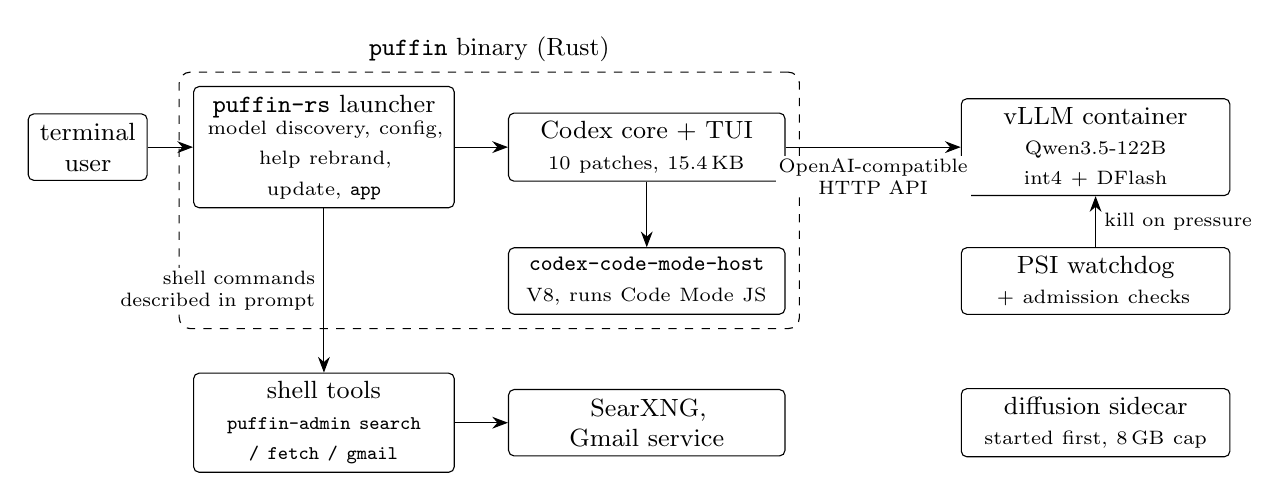
\begin{tikzpicture}[
  box/.style={draw, rounded corners=2pt, align=center, font=\small, inner sep=3pt,
              minimum height=2.4em, text width=#1},
  box/.default=2.6cm,
  grp/.style={draw, dashed, rounded corners=4pt, inner sep=5pt},
  lbl/.style={font=\scriptsize, fill=white, inner sep=1pt},
  >={Stealth[length=2mm]}]
  % row 1: the request path
  \node[box=1.3cm]  (user)     at (-0.2,0)  {terminal\\user};
  \node[box=3.1cm]  (launcher) at (2.8,0)   {\code{puffin-rs} launcher\\\scriptsize model discovery, config,\\help rebrand, update, \code{app}};
  \node[box=3.3cm]  (codex)    at (6.9,0)   {Codex core + TUI\\\scriptsize 10 patches, 15.4\,KB};
  \node[box=3.2cm]  (vllm)     at (12.6,0)  {vLLM container\\\scriptsize Qwen3.5-122B int4 + DFlash};
  % row 2
  \node[box=3.3cm]  (host)     at (6.9,-1.7)  {{\footnotesize\code{codex-code-mode-host}}\\\scriptsize V8, runs Code Mode JS};
  \node[box=3.2cm]  (watch)    at (12.6,-1.7) {PSI watchdog\\\scriptsize + admission checks};
  % row 3
  \node[box=3.1cm]  (tools)    at (2.8,-3.5)  {shell tools\\\scriptsize\code{puffin-admin search / fetch / gmail}};
  \node[box=3.3cm]  (svc)      at (6.9,-3.5)  {SearXNG,\\Gmail service};
  \node[box=3.2cm]  (diff)     at (12.6,-3.5) {diffusion sidecar\\\scriptsize started first, 8\,GB cap};
  % the binary
  \begin{scope}[on background layer]
    \node[grp, fit=(launcher)(codex)(host), label={[font=\small]above:\code{puffin} binary (Rust)}] {};
  \end{scope}
  \draw[->] (user) -- (launcher);
  \draw[->] (launcher) -- (codex);
  \draw[->] (codex) -- (host);
  \draw[->] (codex) -- node[lbl, below=3pt, align=center] {OpenAI-compatible\\HTTP API} (vllm);
  \draw[->] (watch) -- node[lbl, right=2pt] {kill on pressure} (vllm);
  \draw[->] (launcher) -- node[lbl, left=2pt, align=right] {shell commands\\described in prompt} (tools);
  \draw[->] (tools) -- (svc);
\end{tikzpicture}
\caption{Puffin at run time. The only Codex code paths that differ from upstream are the hooks
applied by the patch series; everything Puffin-specific lives in the linked \code{puffin-rs}
crate or in separate local services.}
\label{fig:overview}
\end{figure}

\Cref{fig:overview} shows the running system. The user types \code{puffin}, a single Rust binary.
Before Codex parses its command line, the linked launcher crate runs several steps. It finds the
local vLLM server and waits for it if it is still loading. It asks the server which model it serves
and how long that model's context is. It writes the model catalogue and configuration Codex needs.
Finally it prepends the options that point Codex at the local provider. From then on the process is
Codex, and every upstream flag and subcommand behaves as documented, apart from the cloud surfaces
listed in \cref{sec:cloud}.

Web search, page fetching and Gmail reading are provided by \code{puffin-admin}, the Python
management CLI. The agent invokes them as shell commands (\cref{sec:local}). The same
\code{puffin-admin} manages the vLLM container, a small diffusion-model sidecar, a browser chat UI
built on Onyx \cite{onyx}, and the build of \code{puffin} itself.

\section{A patch-minimal fork}
\label{sec:fork}

\subsection{Build pipeline}

Codex is vendored as a git submodule of our own GitHub fork, pinned to the stable tag
\code{rust-v0.158.0}. The submodule is \emph{never modified}: every test run asserts that
\code{git status} inside it is empty. A build proceeds in six steps.
\begin{enumerate}
  \item Export the pinned commit's \code{codex-rs/} directory with \code{git archive} into a scratch
    tree.
  \item Copy the launcher crate, which is ordinary source in our repository, into that tree as
    \code{codex-rs/puffin}.
  \item Apply the patch series with \code{git apply -{}-check} and then \code{git apply}, so a patch
    that no longer fits fails before anything is half-applied.
  \item Build \code{puffin} and \code{codex-code-mode-host} with Cargo, into a persistent target
    directory. A persistent target means an edit recompiles only the crates it touches.
  \item Install both binaries side by side, because Codex locates the Code Mode host next to its own
    executable. Symlink \code{\textasciitilde/.local/bin/puffin} to the installed binary.
  \item Record a \emph{build key}: a hash of the submodule commit, every patch's bytes, the launcher
    sources and the compiler-profile overrides. An unchanged key skips the build.
\end{enumerate}

Moving to a new upstream release means bumping the submodule and resolving whichever hunks stop
applying. Because the hunks are few and small, conflicts are local and obvious.

\subsection{From 406\,KB to 15\,KB}

The first working series had four patches totalling 406{,}116 bytes. \Cref{tab:patches} shows the
current one. Four techniques made the difference.

\paragraph{Rename at run time, not in the tree.} 395{,}156 bytes of the original series came from a
single patch renaming the agent in Codex's bundled model catalogue (\code{models.json}). That file
stores each system-prompt template, about 20\,KB, as one JSON line, so a one-word change produces a
whole-line diff. The launcher now reads the bundled catalogue through the upstream crate's public
function (\code{bundled\_models\_response}). It takes the longest template, replaces the identity
sentence, which also names a model Puffin does not run, and hands the result to Codex in the model
catalogue it writes anyway. The patch disappeared.

\paragraph{Rewrite presentation where it is assembled.} Help text is spread across doc comments in
dozens of files. Patching each string would grow with every upstream release. Instead, one hook
routes Codex's argument parsing through a function in the launcher crate. That function walks the
\code{clap} command tree once, rewrites the product name in every \code{about}, \code{help} and
\code{bin\_name}, and then parses. It leaves paths and identifiers that merely contain the name,
such as \code{\textasciitilde/.codex}, \code{\$CODEX\_HOME} and \code{codex-code-mode-host}, unchanged,
because renaming them would describe files that do not exist. Only literal usage strings that clap
does not expose remain in the patch.

\paragraph{Use the build system's own unification.} Upstream vendors OpenSSL only for musl targets,
so a glibc build needed system headers, and we had patched \code{codex-core}'s manifest to change
that. Cargo unifies a dependency's features across the whole build graph. A single
\code{openssl-sys = \{features = ["vendored"]\}} line in \emph{our} crate's manifest therefore
applies to every crate that links OpenSSL, and that patch disappeared too. Similarly, a path
dependency located inside the workspace root makes the launcher a workspace member without editing
the workspace manifest, and the binary is renamed at install time rather than in Cargo metadata.

\paragraph{One line per behaviour.} What remains is mostly one-line hooks, as
\cref{tab:patches} shows. Examples: return \code{false} from a slash command's visibility predicate,
mark a subcommand \code{hide = true}, or send a subcommand's dispatch into the launcher. The
largest remaining hunks are presentation strings (patch 0001) and \code{/usage} (0011), which
repurposes a ChatGPT-plan screen as local token statistics.

\begin{table}[t]
\centering
\small
\begin{tabularx}{\linewidth}{@{}l r r X@{}}
\toprule
Patch & Files & $+/-$ & Purpose \\
\midrule
0001 brand-puffin-name & 8 & 20/19 & Product name in TUI header, status card, \code{exec} banner, fixed usage strings \\
0002 puffin-launcher-hook & 2 & 2/1 & One dependency line; route argv through the launcher \\
0005 hide-openai-login & 2 & 4/0 & Hide \code{login}/\code{logout} and \code{/logout} \\
0006 hide-cloud & 1 & 2/1 & Hide \code{cloud} (kept for a private cloud) \\
0007 hide-remote-control & 1 & 2/0 & Hide \code{remote-control} \\
0008 puffin-update & 1 & 2/2 & Send \code{update} to the launcher's release updater \\
0009 remove-feedback & 2 & 3/1 & Remove \code{/feedback} (uploads session logs) \\
0010 hide-voice & 1 & 2/1 & Hide \code{/voice} (hosted realtime API) \\
0011 usage-token-stats & 4 & 7/17 & \code{/usage} shows local token statistics \\
0012 hide-auto-review & 1 & 2/0 & Hide \code{/approve} (defaults to a hosted review model) \\
\midrule
Total (10 patches, 15{,}389 bytes) & 14 & 46/42 & against 4{,}894 Rust files, 1.93M lines \\
\bottomrule
\end{tabularx}
\caption{The patch series at the time of writing. Numbers 0003 and 0004 were retired when their
content moved into the launcher crate.}
\label{tab:patches}
\end{table}

\subsection{Build-reproducibility details}

Three upstream build assumptions did not hold outside OpenAI's release pipeline.
\begin{itemize}
  \item \textbf{V8 flavour.} Code Mode links V8 built with pointer compression and the V8 sandbox.
    The \code{v8} crate's build script downloads a matching prebuilt library \cite{rustyv8}, but that
    flavour is not published for \code{aarch64-unknown-linux-gnu}, so the download fails. OpenAI
    publishes it on its own release page, and the submodule carries a manifest of those files'
    SHA-256 digests. Our builder fetches the archive and its bindings, verifies each against the
    committed manifest, and passes them to Cargo, which mirrors upstream's CI.
  \item \textbf{Lockfile versions.} Upstream's \code{Cargo.lock} records the 158 workspace crates at
    version \code{0.0.0}, which its release job bumps just before building. A \code{-{}-locked} build
    therefore fails. The only entries Cargo rewrites are those 158 workspace versions, so we build
    without \code{-{}-locked} and have confirmed that every third-party pin is unchanged.
  \item \textbf{Debug information.} The upstream release profile keeps line tables and strips only
    at packaging. Built as-is, the agent binary was 1.4\,GB. Setting
    \code{CARGO\_PROFILE\_RELEASE\_DEBUG=none} and \code{\_STRIP=debuginfo} through the environment,
    which needs no patch, yields 315\,MB. This also matters at run time
    (\cref{sec:local}).
\end{itemize}

\section{Cutting the cloud cord}
\label{sec:cloud}

We audited every subcommand and slash command of Codex 0.158.0 for a dependency on OpenAI-hosted
services. \Cref{tab:cloud} lists what we changed. We used four treatments, deliberately
distinguished:
\begin{itemize}
  \item \emph{Refuse}: the launcher rejects the command before Codex parses it, with an explanation.
  \item \emph{Hide}: the command is removed from help and menus, but its code stays compiled for a
    future private-cloud implementation.
  \item \emph{Replace}: the same command does something local.
  \item \emph{Remove}: the command is invisible and unreachable.
\end{itemize}
Hiding alone is not a security boundary: a hidden clap subcommand still parses. Commands that
initiate an OpenAI sign-in or reach OpenAI's servers are therefore also refused in the launcher.
The launcher currently checks only the first argument, so \code{puffin -c k=v cloud} would evade
the refusal. This is a known gap, and fixing it means scanning for the first non-option argument.

\begin{table}[t]
\centering
\small
\begin{tabularx}{\linewidth}{@{}l X l@{}}
\toprule
Surface & Why it does not fit an air-gapped agent & Treatment \\
\midrule
\code{login}, \code{logout}, \code{/logout} & ChatGPT / API-key sign-in; no account exists & refuse + hide \\
\code{cloud}, \code{cloud-tasks} & Browses tasks on OpenAI's servers & refuse + hide \\
\code{remote-control} & Relays sessions through OpenAI's servers & hide \\
\code{update} & Installs upstream Codex over Puffin & replace (verified release download) \\
\code{/feedback} & Uploads session logs to OpenAI & remove \\
\code{/voice} & OpenAI realtime voice API & hide \\
\code{/usage} & ChatGPT plan usage and limit resets & replace (local token statistics) \\
\code{/approve} (auto-review) & Defaults to a hosted review model & hide \\
\code{app} & Opens OpenAI's closed-source desktop app & replace (opens Puffin's own window) \\
update check at start-up & Compares against \code{openai/codex} releases & disabled in config \\
\bottomrule
\end{tabularx}
\caption{Cloud-coupled surfaces and their treatment. On Linux, Codex's \code{app} subcommand is
not compiled at all, so Puffin's \code{app} is new.}
\label{tab:cloud}
\end{table}

\paragraph{Updates.} \code{puffin update} replaces Codex's installer-detection logic. It queries the
latest \emph{published} release of Puffin's repository, compares it with the version stamped into
the binary at release build time, and downloads the gzipped \code{puffin} and
\code{codex-code-mode-host} with a SHA-256 manifest. It verifies both files before replacing either,
and swaps them in next to the running executable, so a failed download leaves the installation
intact. A release workflow builds these binaries on an arm64 runner. We note one operational hazard
in \cref{sec:lessons}: a release that went out without the binaries.

\section{Running a vendor agent against a local model}
\label{sec:local}

\paragraph{Discover, do not configure.} The local server's model can change between sessions, and
an earlier version of our launcher left Codex advertising the previous model with the wrong context
length. vLLM's \code{/v1/models} endpoint reports both the served model's identifier and its
\code{max\_model\_len}. The launcher therefore derives the model catalogue entry from the running
server, with no copy of the model registry: context window, auto-compaction limit and truncation
policy all come from that value.

\paragraph{The catalogue is a hard schema.} Codex refuses a model it has no catalogue entry for, and
parses entries with strict \code{serde} structs. A wrongly shaped field is a start-up failure, not
an ignored key. Several fields have non-obvious shapes:
\begin{itemize}
  \item reasoning levels are \code{\{effort, description\}} records;
  \item \code{visibility} is one of \code{list|hide|none};
  \item truncation is \code{\{mode, limit\}};
  \item \code{base\_instructions} is required in practice, and it is the \emph{entire} system prompt,
    not a label.
\end{itemize}
An early version filled \code{base\_instructions} with a one-line placeholder. The model then had no
description of its tools, guessed tool names that do not exist, and fell back to \code{curl} for
work a tool was provided for. Supplying Codex's own template, with the identity sentence rebranded,
fixed this.

\paragraph{Configuration scoping.} Codex's \code{config.toml} accumulates tables written by Codex
itself, for example \code{[tui.model\_availability\_nux]}. Appending a top-level key such as
\code{model\_catalog\_json = "..."} to such a file silently makes it a member of the last table. The
result is the start-up error \emph{invalid type: string, expected u32}. The same failure recurred
later with a different table. The launcher now edits the file as a syntax tree
(\code{toml\_edit}). It sets keys that must follow the server unconditionally, and adds keys that
the user may override only when they are absent.

\paragraph{Tools as shell commands, not MCP.} Code Mode exposes MCP tools only inside its JavaScript
runtime, as \code{tools.mcp\_\_server\_\_tool(args)}. We wired a SearXNG \cite{searxng} MCP server
for web search. The server initialised and its tools reached the model's context, but the local
model repeatedly called the namespace directly, received \emph{unsupported call}, and gave up.
Plain shell commands described in the system prompt worked reliably:
\code{puffin-admin search}, \code{fetch} and, later, \code{gmail search|read|status}. This is one
model on one harness and should not be over-generalised. Still, it suggests that for local models,
the tool surface a vendor harness assumes may need to be flattened back into the shell.

\paragraph{Untrusted content.} Email gives an agent that holds a shell a prompt-injection channel.
Gmail access is read-only by construction. \code{gmail read} frames every message between
\emph{BEGIN EMAIL (untrusted)} and \emph{END EMAIL} markers, and the prompt section is added only when
an account is connected, and states that email content is never instructions. We regard these as
mitigations, not a defence.

\paragraph{Binary size is prompt latency.} The pre-rewrite launcher recovered Codex's prompt by
scanning the installed binary for JSON-escaped templates. At 1.4\,GB this took about 0.77\,s per
launch, and 0.2\,s after stripping. Reading the template through the crate's API removed the scan
entirely.

\section{Host safety on unified memory}
\label{sec:safety}

With no dedicated GPU memory, a model load competes with the desktop for every page. We learned
this the hard way. On 14~August~2026, six loads in one hour took the workstation down hard enough to
need the power button. None of the freezes invoked the kernel OOM killer. Driver-pinned pages are
unreclaimable, and they are not charged to any process the killer would select, so the kernel spun
in direct reclaim instead of killing anything. Puffin's server manager now enforces two layers.

\paragraph{Admission checks (before a load).} All conditions are checked and reported together,
because each fix needs its own \code{sudo}.
\begin{itemize}
  \item \emph{An OOM handler} (systemd-oomd or earlyoom) acts on pressure-stall information
    \cite{linuxpsi} before the livelock forms.
  \item \emph{At least 64\,GB of swap} gives the kernel somewhere to put cold anonymous pages.
  \item \code{vm.min\_free\_kbytes} \emph{at 1\,GiB or more}. The stock value is about 44\,MB on
    this machine, which a loader reading gigabytes per second exhausts between reclaim passes.
  \item \code{vm.watermark\_scale\_factor} \emph{at 200 or more}, so background reclaim starts
    earlier.
  \item \emph{sysstat installed}, because its history is the only pressure record that survives a
    hard reset.
\end{itemize}
The container is also nominated as the preferred OOM victim (\code{oom\_score\_adj}\,=\,800).

\paragraph{Watchdog (during a load).} A thread samples \code{/proc/pressure/memory} once per second.
It resolves the container's cgroup and kills the container on either of two rules:
\begin{itemize}
  \item the ``full'' stall share over 10\,s stays at or above 60\% for 5\,s, matching systemd-oomd's
    default limit;
  \item the 60\,s average reaches 25\%.
\end{itemize}
The second rule catches pressure that oscillates around the first threshold, resets its timer on
every dip, and grinds indefinitely. The kill has three paths, tried in the order the host can still
afford:
\begin{enumerate}
  \item a direct \code{SIGKILL} to the cgroup's processes, which needs privileges the tool normally
    lacks;
  \item a single request over Docker's Unix socket, with no fork;
  \item the Docker CLI, last, because forking a Go binary is the work least likely to be scheduled
    during a reclaim livelock.
\end{enumerate}

\paragraph{Consequences for serving.} These margins are why the model runs at a 32k context rather
than 131k: a longer context was refused at start-up for want of 3.3\,GiB of KV cache. They also
fix the order of start-up. The diffusion sidecar starts \emph{before} vLLM, with a fixed 8\,GB
cgroup cap, because vLLM's pre-flight reads current free memory. A resident sidecar is accounted
for, whereas the reverse order lets a marginal check pass and then lose the memory mid-load.
Every heavy background job we have added since runs under
\code{systemd-run -p MemoryMax=\ldots{} -p MemorySwapMax=0}. Code indexing, for example, uses a cap,
so exhaustion kills the job instead of the host (\cref{sec:index}).

\section{Evaluation}
\label{sec:eval}

We evaluate what the system does today. We have \emph{not} yet measured task-level coding accuracy,
for example on SWE-bench \cite{jimenez2024swebench}. \Cref{sec:limits} discusses this.

\begin{table}[t]
\centering
\small
\begin{tabular}{@{}l r@{}}
\toprule
Metric & Value \\
\midrule
Upstream (Codex \code{rust-v0.158.0}) & 4{,}894 Rust files, 1.93M lines \\
Patch series, initial $\rightarrow$ current & 406{,}116 B (4 patches) $\rightarrow$ 15{,}389 B (10 patches) \\
Upstream files touched / lines changed & 14 files / $+46,\ -42$ \\
Launcher crate (\code{puffin-rs}) & 1{,}403 lines, 24 unit tests \\
Agent binary, unstripped $\rightarrow$ stripped & 1.4\,GB $\rightarrow$ 315\,MB (+ 93\,MB Code Mode host) \\
Incremental rebuild after a launcher edit & $\approx$7 min (thin LTO relink) \\
Management and services (Python) & 79 modules, 19.7k lines; 380 tests \\
\quad without a model server & 317 pass, 63 skip (need live server) \\
Live slash-command suite (local 122B model) & 70 tests: 65 pass, 3 fail, 2 skip; 731.6\,s \\
Decode throughput, single stream, 32k context & prose 23.8 / code 49.9 / JSON 53.1 tok/s \\
\bottomrule
\end{tabular}
\caption{Measurements on one GB10 (128\,GB). Throughput is from the model registry's benchmark
record for the default configuration, not re-measured for this paper.}
\label{tab:eval}
\end{table}

\paragraph{Live slash-command suite.} A test drives every slash command of the pinned Codex source
on a pseudo-terminal, in a throwaway git repository and \code{CODEX\_HOME}, against the running
local model. It asserts per command that the expected screen or reply appears, and that removed
commands are rejected. \Cref{tab:eval} gives the totals. Two commands that upstream labels ``DO NOT
USE'' are skipped. The three failures were diagnosed from session transcripts.
\begin{enumerate}
  \item \code{/init}: the harness treated the brief disappearance of the ``esc to interrupt'' marker
    between tool calls as the end of a turn. It checked for \code{AGENTS.md} too early, and its
    clean-up interrupted a model that was working normally. This is a harness bug.
  \item \code{/btw}: this is an alias of \code{/side}, which is unavailable until a conversation
    exists. The test must converse first. This is also a harness bug.
  \item \emph{Fresh-home start}: with an empty configuration directory, \code{puffin} opens on
    Codex's ``Sign in with ChatGPT'' screen instead of the composer, even though the launcher has
    written a complete local-provider configuration. This is a real defect, and it would be the
    first thing a new user sees. Fixing it requires suppressing Codex's first-run onboarding for the
    local provider.
\end{enumerate}

\paragraph{Throughput.} Speculative decoding helps structured output most. JSON and code, being
predictable, accept long DFlash drafts: 49.9 and 53.1 tokens/s against 23.8 for prose. That
distribution suits an agent whose output is dominated by tool calls and code.

\section{Towards compiler-exact code navigation}
\label{sec:index}

Today the agent navigates with \code{rg} and file reads. On the 4{,}894-file upstream workspace this
costs many rounds, and it silently misses calls through traits, generics and re-exports. We surveyed
open-source code-intelligence tools with the constraints of an air-gapped AGPL product in mind. The
constraints were a compatible licence, no network or telemetry, Rust and Python support, and arm64
availability. We selected a two-layer design, now specified in the repository.
\begin{itemize}
  \item \emph{Universal layer}: codebase-memory-mcp \cite{codebasememorymcp,vogel2026codebasememory}.
    It is a single MIT-licensed C binary with 158 tree-sitter \cite{treesitter} grammars and a code
    embedding model compiled in. It builds a call graph and supports semantic search. Its authors
    report approximate type resolution, with a target of about 95\% on idiomatic Python.
  \item \emph{Exact layer}: SCIP \cite{scip} indexes produced by compiler front-ends, such as
    rust-analyzer and Pyright-based \code{scip-python}, for projects that build.
\end{itemize}
A router in the launcher answers each question from the better layer. It joins the two through the
definition's location, which maps a qualified name to an opaque SCIP symbol. It tags every result
\emph{exact} or \emph{heuristic}, and reports calls it could not resolve. The agent's prompt then
requires verification whenever a result is heuristic or unresolved and the change is a rename,
signature change or deletion. This follows the graph-guided localisation idea of LocAgent
\cite{chen2025locagent} and the multi-view serving of CodeNib \cite{yu2026codenib}, specialised to a
single air-gapped machine.

The first attempts to index the upstream workspace with \code{rust-analyzer scip} under an 8\,GB
cgroup cap were OOM-killed within the cap. The host was unaffected. Before indexing, the indexer compiles and runs the
workspace's build scripts and procedural macros, of which several hundred were loaded before the
kill. The same fact is why the design indexes only trusted repositories and runs indexers in a
network-less sandbox. The memory cost of exact indexing
on a workspace of this size is an open measurement. It will decide whether exact indexing can run
beside a resident 122B model at all.

\section{Lessons}
\label{sec:lessons}

\paragraph{Keep the fork boring.} Every behaviour that could live in a linked crate went there.
Every remaining hook is a single call or predicate. The measure of success is how long an upstream
bump takes, not how little code we wrote. A 15\,KB series that touches 14 files turns an upstream
release into an afternoon's review rather than a merge project.

\paragraph{Presentation diffs are the expensive ones.} Almost all of the original series' size, 97\%,
was a one-word rename inside machine-formatted data. Renaming at run time, or at the point where
presentation is assembled, removed it. We expect this to be the common case for rebranded forks.

\paragraph{Local models change the tool contract.} A harness tuned for a frontier hosted model
exposes tools in ways a smaller local model may not use. It is cheaper to adapt the tool surface to
the model, here by using shell commands, than to wait for the model to adapt to the surface.

\paragraph{Unified memory needs admission control, not just limits.} A container memory cap bounds
the container. It does not decide who dies when the host runs short, and it does not prevent a
reclaim livelock in which nothing dies. Pre-flight checks, pressure-based watchdogs and caps on
every auxiliary job were all necessary.

\paragraph{Parallel automation needs the same discipline as parallel humans.} Much of this system
was built with an AI coding assistant running several sub-tasks concurrently in one working tree.
Three failure modes appeared that are familiar from team development, in faster form.
\begin{itemize}
  \item Concurrent builds wiped each other's shared source tree. A file lock in the builder fixed
    this.
  \item A copy that preserved file timestamps let Cargo link a stale launcher. Copying with fresh
    timestamps fixed this.
  \item Commits swept up another task's staged changes, in one case deleting the patch series from
    a commit. Checking the index before every commit and staging only named hunks prevented
    recurrences.
\end{itemize}
Separately, a stopped release task had already triggered a workflow that published a release
without the agent binaries. It was cancelled too late and then deleted. Outward-facing actions
started by automation need their own kill switch.

\section{Related work}

Research agents such as SWE-agent \cite{yang2024sweagent} and OpenHands \cite{wang2024openhands}
study the agent-computer interface and evaluate on SWE-bench \cite{jimenez2024swebench}. They can
point at local models, but they are research harnesses rather than hardened daily-use clients.
Terminal assistants such as Aider \cite{aider} and Goose \cite{goose} support local models natively.
Our contribution is complementary. We show how to take a vendor's production client, keep it
upgradable, and make it local and self-contained. Code-navigation work for agents, including
LocAgent's code graphs \cite{chen2025locagent}, CodeNib's multi-view context serving
\cite{yu2026codenib} and tree-sitter knowledge graphs served over MCP \cite{vogel2026codebasememory},
informs \cref{sec:index}. On the serving side we rely on vLLM's paged attention \cite{kwon2023vllm},
speculative decoding \cite{leviathan2023speculative} and block-diffusion drafting
\cite{chen2026dflash}. Our contribution there is the host-level safety that unified memory requires,
rather than any serving algorithm.

\section{Limitations}
\label{sec:limits}

\begin{itemize}
  \item \textbf{No task-level accuracy.} We have not run SWE-bench or a comparable benchmark, so we
    make no claim about how well Puffin solves tasks relative to hosted Codex or to other local
    agents. This is the most important missing measurement.
  \item \textbf{One machine, one model.} All results come from a single GB10 with one model
    configuration. The tool-calling observation in \cref{sec:local} is anecdotal evidence from that
    configuration.
  \item \textbf{Throughput is not re-measured.} The throughput figures come from the system's own
    benchmark record at the time the default model was chosen.
  \item \textbf{Known open defects:} the first-run sign-in screen (\cref{sec:eval}) and the
    first-argument-only refusal check (\cref{sec:cloud}).
  \item \textbf{Code index not built.} The code-index design is specified but not implemented. Its
    key memory measurement is open.
\end{itemize}

\section{Conclusion}

Puffin shows that a production coding-agent client can be made fully local on a single
unified-memory workstation without giving up the ability to take upstream releases. The fork adds
15.4\,KB of hooks to a 1.93M-line codebase. The localisation lives in a separate crate, the cloud
surface is audited and neutralised explicitly, and the host is protected by admission checks and a
pressure watchdog. The next steps are a task-level accuracy evaluation, the fix for first-run
onboarding, and the two-layer code index.

\section*{Availability}
The system is developed in a private repository at the time of writing. The patch series, launcher
crate, builder and specifications described here are licensed AGPL-3.0-or-later. Codex is used
under its upstream licence.

\section*{Acknowledgements and disclosure}
Much of the implementation, and drafts of this manuscript, were produced with the assistance of
an AI coding assistant (Anthropic's Claude) working under the author's direction. The author
reviewed the system and this text and takes responsibility for them. All numbers in this paper
were measured on the author's machine or read from the repository, and each arXiv citation was
checked against the arXiv record.

\bibliographystyle{plainnat}
\bibliography{references}

\end{document}
